\Chapter{Parallel computing}{Employing a thousand monkeys}
\label{chap:Parallel computing}

\begin{quote}\small
  \emph{``Here be dragons.''}
\end{quote}

If you have a multicore processor, or even multiple processors or machines available, one obvious way to speed up your code is to employ multiprocessing.
However, this is a difficult and dangerous endeavor, especially if you don't have any prior experience.
Parallel programs are far more difficult to write and debug than sequential ones, mostly because concurrency introduces entire classes of potential bugs, like race conditions and deadlocks.
Also, even if it does work, it's not always beneficial.
Some algorithms simply don't scale to multiple processors.
\begin{marginfigure}
  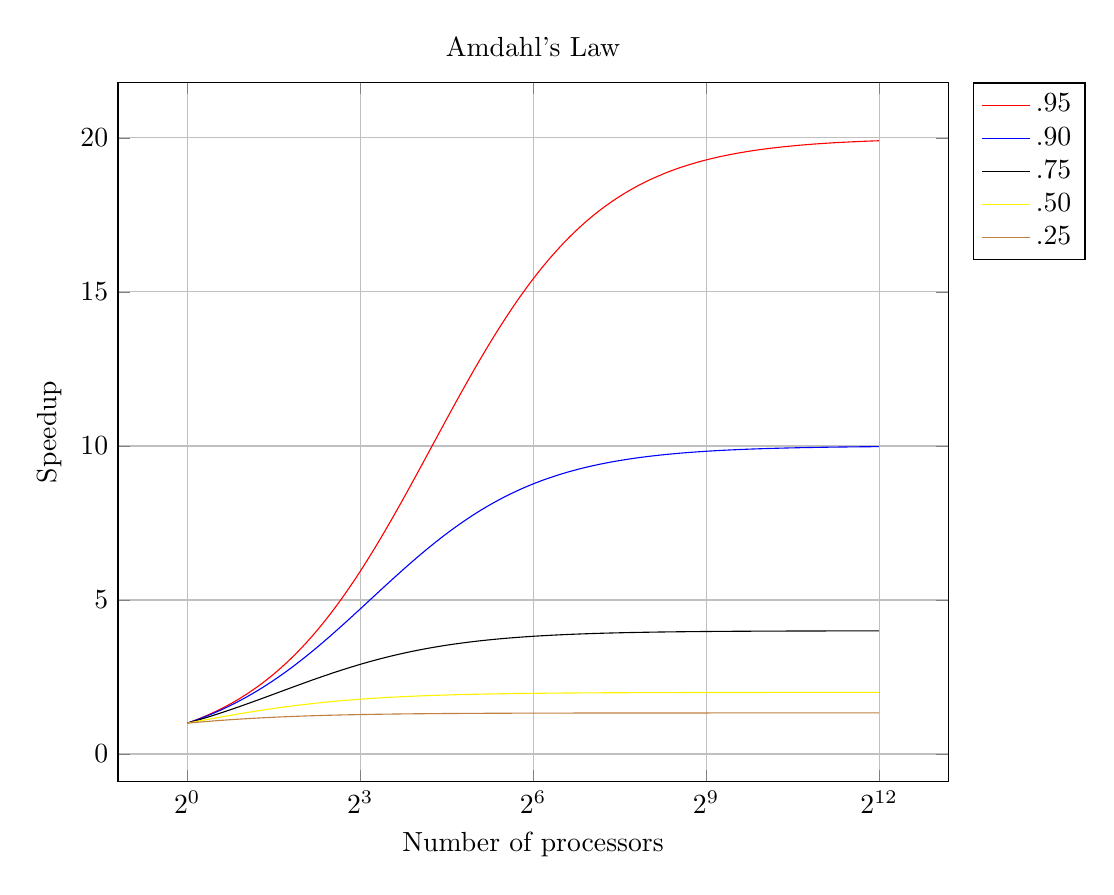
\begin{tikzpicture}
    \begin{axis}[
      title=Amdahl's Law,
      width=\textwidth,
      grid=major,
      xlabel=Number of processors,
      xmode=log,
      log basis x={2},
      xtick={1,8,64,512,4096},
      ylabel=Speedup,
      ylabel near ticks,
      ytick={0,5,10,15,20},
      legend pos=outer north east,
      cycle list name=color list
    ]
    \foreach \p in {.95, .90, .75, .50, .25} {
      \addplot+[
        no marks,
        domain=1:4096,
        samples=201
      ] {1/((1 - \p) + \p/x)};
      \addlegendentryexpanded{$\p$};
    }
    \end{axis}
  \end{tikzpicture}
  \caption{\index{Amdahl's Law}Amdahl's law details the theoretical speedup of a fixed-size algorithm given the fraction of the algorithm that can execute in parallel and the number of processors available for computation.}
\end{marginfigure}
Despite its complexity, parallel programming is unavoidable in high-performance computing.
While a true introduction is outside the scope of these notes, we'll give a few guidelines that might help you from accidentally shooting yourself in the foot:
\begin{itemize}
  \item\textbf{Make sure your program works first.} Although this is true for optimizations in general, it is doubly so for parallel programs.
    Programs are much harder to debug when they run in parallel, so leave parallelization for the final step.
  \item\textbf{Check whether the bottleneck in your program benefits from parallelization.} Not every algorithm scales well.
    It would be a waste of time to spend effort parallelizing your code only to discover that it's now actually slower.
  \item\textbf{Use OpenMP.}\footnote{OpenMP is available for C, \Cplusplus, and Fortran.
    If you are using \Cplusplus, the \emph{Intel Threading Building Blocks} library is a possible alternative; it has high-level support for certain algorithms and data structures.} For ICCP you won't be using supercomputers or systems with multiple nodes.
    Sophisticated libraries like MPI\footnote{Message Passing Interface: a standardized protocol for communications between nodes in a cluster---used on pretty much every supercomputer in the TOP500.} are overkill and introduce needless complexity.
    OpenMP only works on single machines with shared memory, but it is by far the easiest framework to use.
    All you need to do is add \texttt{-fopenmp} to \texttt{FFLAGS} and \texttt{LDFLAGS} in your \texttt{Makefile} and add a few directives to your code.
    For example
\begin{lstlisting}[caption=, nolol]
  !$omp parallel do
  do i = 1, n
      y(i) = x(i) * i
  end do
  !$omp end parallel do
\end{lstlisting}
    will execute the loop in parallel. Use Google for more information on how to use OpenMP.
  \item\textbf{Don't use more threads than you have physical cores.} This may seem like stating the obvious, but it actually happens rather often.
  Most modern Intel processors implement hyper-threading.
  This doubles the apparent number of cores, which helps with task switching when you're running many different programs at once.
  However, for CPU intensive calculations, like the ones you'll be running, the threads will be competing for the available physical cores.
  In that case doubling the number of threads will actually harm performance.
\end{itemize}

